\documentclass{article}

\usepackage{ucs}

\usepackage[utf8x]{inputenc}
\usepackage[greek, english]{babel}
\usepackage{alphabeta}
\usepackage{lmodern}

\usepackage[linguistics]{forest}

\usepackage{listings}

\usepackage{graphicx}
\graphicspath{./images/}

\usepackage{forest}

\title{Δεύτερο μέρος εργαστηριακής εργασίας στο μάθημα Τεχνητής Νοημοσύνης}
\date{2021-01-15}
\author{Ιάκωβος Μαστρογιαννόπουλος}

\definecolor{codegreen}{rgb}{0,0.6,0}
\definecolor{codegray}{rgb}{0.5,0.5,0.5}
\definecolor{codepurple}{rgb}{0.58,0,0.82}
\definecolor{backcolour}{rgb}{0.95,0.95,0.95}

\lstdefinestyle{mystyle} {
    backgroundcolor=\color{backcolour},
    commentstyle=\color{codegreen},
    keywordstyle=\color{magenta},
    numberstyle=\tiny\color{codegray},
    stringstyle=\color{codepurple},
    basicstyle=\ttfamily\footnotesize,
    breakatwhitespace=false,
    breaklines=true,
    captionpos=b,
    keepspaces=true,
    numbers=left,
    numbersep=5pt,
    showspaces=false,
    showstringspaces=false,
    showtabs=false,
    tabsize=2
}

\lstset{style=mystyle}


\begin{document}
    \pagenumbering{gobble}
    \maketitle

    \newpage
    \tableofcontents
    \newpage
    \lstlistoflistings

    \newpage
    \begin{abstract}
        Αυτό είναι το δεύτερο μέρος της εργαστηριακής εργασίας του μαθήματος Τεχνητής Νοημοσύνης του
        Ιάκωβου Μαστρογιαννόπουλου, AM: cse 242017102 εξάμηνο 7.  
    \end{abstract}

    \newpage
    \pagenumbering{arabic}
    \section{Πρόλογος}

    \paragraph{}
    Στη συγκεκρίμενη εργασία του μαθήματος <<Τεχνητής Νοημοσύνης>> είχαμε να μελετήσουμε το προβλήμα του parking. Βέβαια,
    για να μπορέσουμε να φτάσουμε στο σημείο της υλοποίησης του κωδικά, πρώτα πρέπει να εξηγηθούν μερικά πραγμάτα με το ποιο είναι
    το πρόβλημα, πώς μπορούμε να το υλοποιήσουμε και ποια θα είναι τα πιθανά αποτελέσματα που θα μπορούσαμε να πάρουμε πίσω.  
    Σε αυτό το μέρος χρησιμοποιήθηκε το εργαλείο της Clips.

    \newpage
    \section{Κατανοήση προβλήματος - Πρόβλημα του Parking}
    \paragraph{}
    Όπως και στο πρώτο μέρος της εργασίας, το πρόβλημα που έχουμε να λύσουμε είναι το πρόβλημα του Parking. Θεωρετηκά, υπάρχει ένας αυτόματος οδηγός ο οποίος προσπαθεί να βρει
    ελευθέρο χώρο για να γεμίσει τα αμάξια που θέλουν να μπουν μέσα στο Parking. Υπάρχουν Ν spaces από τα οποία θα μπορούσαν μερικά από αυτά
    να ήταν τελείως άδεια, ενώ κάποια αλλά να είχαν μια πλατφόρμα. Στο δεύτερο μέρος της εργασίας, όμως υπάρχουν και επιπλέον όροφοι 
    Μ, όπου κάθε Μ όροφος έχει Ν spaces.

    \paragraph{}
    Παρόλο που στο προηγούμενο μέρος χρησιμοποιήθηκαν αλγόριθμοι αναζήτησης για την επιλυσή του, αυτή την φόρα χρησιμοποιούμε εμπείρα συστήματα.
    Ο στόχος όμως δεν αλλάζει, ο όποιος είναι να βρίσκει τις πλατφόρμες και από εκεί να καταλαβαίνει ποιες από αυτές έχουν ελεύθερο χώρο και να τις γεμίζει.
    Ένα εμπείρο συστήμα αποτελείται από κανόνες και γεγονόντα. Στο συστήμα που θα φτιάξουμε θα πρέπει να έχει τα εξής γεγονόντα:

    \begin{itemize}
        \item Τα spaces και οι γειτονικές τους καταστάσεις
        \item Οι πλατφόρμες (platforms)
        \item Το info της τρέχουσας κατάστασης του συστήματος
        \item Και τα αυτοκίνητα που είναι παρκαρισμένα
    \end{itemize}

    \paragraph{}
    Ενώ οι κανονές είναι οι εξής:

    \begin{itemize}
        \item O αρχικός κανόνας που αρχικοποιεί το info και ζητάει να μάθει πόσα αυτοκίνητα είναι στην ουρά και περιμένουν
        \item Οι κανόνες που περιγράφουν πως κουνιέται βορεία, νότια, ανατολικά και δυτικά η πλατφόρμα αναλόγως με τις γειτονικές
            καταστάσεις που έχουν τα spaces
        \item Και ο τελικός κανόνας που λειτουργεί μόνο όταν δεν υπάρχει άλλο αμαξί στην ουρά
    \end{itemize}

    \paragraph{}
    Η εργασία είναι χωρισμένη σε δύο βήματα, όπου θα τα αναλύσουμε ξεχωριστά στο PDF.

    \newpage
    \section{Βήμα 1}
    \subsection{Ζητούμενα πρώτου βήματος}
    \paragraph{}
    Το πρώτο βήμα του δευτέρου μέρους της εργασίας μας ζητάει να φτιάξουμε ένα parking με 6 spaces και 5 πλατφόρμες σε έναν όροφο.
    Έχουμε 6 spaces (s1-s6) όπου η s2 είναι η είσοδος των αυτοκινήτων και στα υπόλοιπα έχουμε από μία πλατφόρμα (p1-p5). 
    Ο αυτόματος παρκαδόρος μπορεί να κινηθεί βόρεια, νοτεία, δυτικά και ανατολικά. Το αυτοκίνητο τοποτεθείται στην πλατφόρμα
    την οποία ήταν άδεια.

    \subsection{Templates πρώτου βήματος}
    \paragraph{}
    Τα templates του πρώτου βήματος είναι η εξής:

    \begin{lstlisting}
        (deftemplate space
            (slot name)
            (slot level)
            (slot state)
        )

        (deftemplate platform
            (slot name)
            (slot space)
            (slot plat_state)
        )

        (deftemplate car
            (slot cars_left)
            (slot state)
        )
    \end{lstlisting}

    \subsection{Γεγονόντα πρώτου βήματος}
    \paragraph{}
    Τα γεγονόντα του πρώτου βήματος είναι η εξής:

    \begin{lstlisting}
        (deffacts space-init
            (space (name s1) (level 1) (state Y))
            (space (name s2) (level 1) (state N))
            (space (name s3) (level 1) (state Y))
            (space (name s4) (level 1) (state Y))
            (space (name s5) (level 1) (state Y))
            (space (name s6) (level 1) (state Y))
        )

        (deffacts plat-init
            (platform (name p1) (space s1) (plat_state E))
            (platform (name p2) (space s3) (plat_state E))
            (platform (name p3) (space s4) (plat_state E))
            (platform (name p4) (space s5) (plat_state E))
            (platform (name p5) (space s6) (plat_state E))
        )

        (deffacts east
            (east s1 s2)
            (east s2 s3)
            (east s4 s5)
            (east s5 s6)
        )

        (deffacts north
            (north s1 s4)
            (north s2 s5)
            (north s3 s6)
        )

        (deffacts west
            (west s2 s1)
            (west s3 s2)
            (west s5 s4)
            (west s6 s5)
        )

        (deffacts south
            (south s4 s1)
            (south s5 s2)
            (south s6 s3)
        )
    \end{lstlisting}

    \newpage
    \subsection{Κανόνες πρώτου βήματος}
    Παμέ να δούμε αναλητικά το κάθε κανόνα ξεχωριστά.

    \subsubsection{Κανόνας εκκίνησης}
    \begin{lstlisting}[caption=Κανόνας εκκίνησης]
; Kanonas pou ksekinaei to programma
(defrule startup
    (declare (salience 100)) ; Dinei protereotita ston kanona
    (initial-fact)
=>
    (set-strategy random)
    (printout t "Starting the program!" crlf)

    (printout t "Enter the ammount of cars waiting in the line." crlf)
    (bind ?c(read)) ; Eisagwgh arithmwn autokitwn pou perimenei sthn oura
    (if (<= ?c 0)
    then
        (printout t "The ammount of cars cannot be 0 or less than 0." crlf)
        (assert (car (cars_left 0) (state GOAL_NOT_FOUND)))
    else
        (assert (car (cars_left ?c) (state GOAL_NOT_FOUND)))
    )
)
    \end{lstlisting}

    \paragraph{}
    Εδώ ο κανόνας παίρνει από τον χρηστη των αριθμό των αυτοκινήτων που περιμένει στην ουρά για να μπουν μέσα.
    Εάν του δωθεί αριθμός μικρότερος ή ισός του μηδενός, τότε έγινε κάποιο λάθος και το πρόγραμμα λήγει εδώ.
    Επιπρόσθετα, όπως είναι και σχολιασμένο, έχει προτερεότητα σε σχέση με άλλους κανόνες και τρέχει πάντα πρώτο.

    \subsubsection{Κανόνας goal\_found}
    \begin{lstlisting}[caption=Κανόνας goal\_found]
(defrule goal_found
    (declare (salience 100))
    ?c<-(car (cars_left 0) (state GOAL_NOT_FOUND))
=>
    (modify ?c (state GOAL_FOUND))
    (printout t "Goal found. End of program." crlf)
)
    \end{lstlisting}

    \paragraph{}
    Ο συγκεκριμένος κανόνας έχει ως όρισμα το car να έχει cars\_left 0 και state GOAL\_NOT\_FOUND. Τότε, και μόνο τότε, αλλάζει το state
    σε GOAL\_FOUND και λήγει εδώ το προγράμμα με το goal να έχει βρεθεί.

    \newpage
    \subsubsection{Τυπικός κανόνας κίνησης}
    \begin{lstlisting}[caption=Τυπικός κανόνας κίνησης]
; Kanonas pou kounaei anatolika ton automato parkadoro
(defrule moveEast
    ?z<-(space (name ?y) (state N)) ; Trexon space
    (east ?x ?y) ; Edw allazei mono
    ?p<-(space (name ?x) (state Y)) ; Space pou tha paei o parkadoros
    ?q<-(platform (space ?x) (plat_state ?ps)) ; Platforma pou uparxei sto space
    ?c<-(car (cars_left ?cars) (state GOAL_NOT_FOUND)) ; Katastasi autokinhtwn
=>
    (modify ?p (state N)) ; Allagi space state se N gia to space pou tha pame 
    (modify ?z (state Y)) ; Allagi space state se Y gia to space pou eimastan
    (if (eq ?ps F)
    then
        (modify ?q (space ?y))
        
    else
        (modify ?q (space ?y) (plat_state F)) ; Ean den einai gemato, vazei to autokinito
        (modify ?c (cars_left (- ?cars 1))) ; Afairei 1 apo ta autokinhta pou apomenoun
    )
)
    \end{lstlisting}

    \paragraph{}
    Αυτός είναι ένας τυπικός κανόνας μετακίνησης του αυτόματου παρκαδόρου (συγκεκριμένα είναι του ανατολικού αλλά δεν αλλάζει πολύ
    ο κάθε κωδικάς). Σαν ορίσματα παίρνει το τρέχον space, το γειτονικό του και την πλατφόρμα, και πρέπει το car να έχει state
    GOAL\_NOT\_FOUND. Στην συνέχεια, θα αλλάξει το state του κάθε space, αφού το ένα θα πάρει την πλατφόρμα του άλλου. Μετά,
    ελέγχει εάν η πλατφόρμα είναι γεμμάτη, τότε απλώς αλλάζει την πλατφόρμα θέση, αλλιώς αλλάζει την πλατφόρμα θέση και
    αλλάζει το state της πλατφόρμας έτσι ώστε να είναι γεμμάτη και να αφαίρει 1 αυτοκίνητο από το car.

    \newpage
    \subsection{Βήμα 1 source code}
    \lstinputlisting[caption=Βήμα 1]{code/parking_simple.clp}

    \newpage
    \subsection{Ενδεικτικά τρεξίματα του πρώτου βήματος}
    \subsubsection{Πριν την εκκίνηση}
    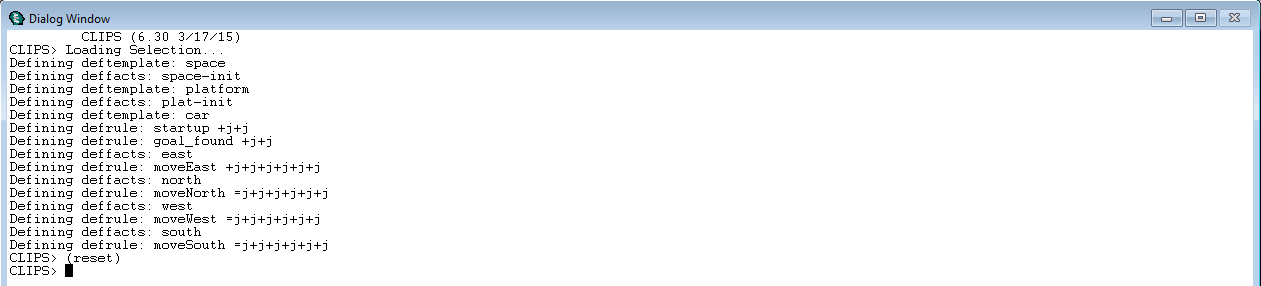
\includegraphics[scale=0.5]{images/dialog_window_b1_1.png}
    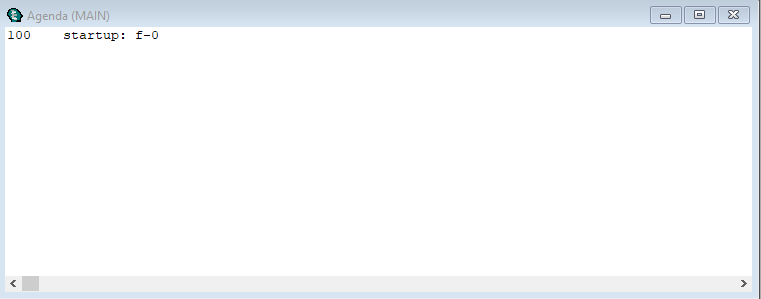
\includegraphics[scale=0.5]{images/agenda_window_b1_1.png}
    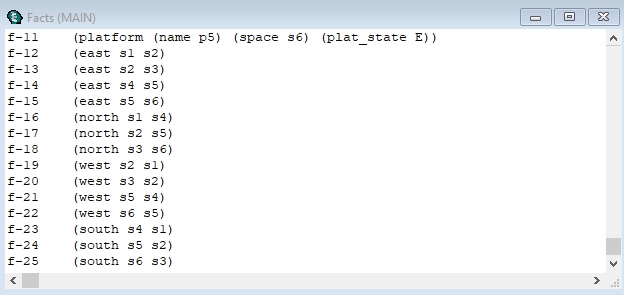
\includegraphics[scale=0.5]{images/facts_window_b1_1.png}

    \newpage
    \subsubsection{Κανόνας εκκίνησης}
    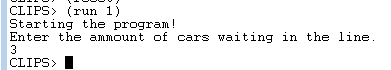
\includegraphics[scale=0.5]{images/dialog_window_b1_2.png}
    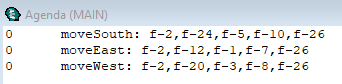
\includegraphics[scale=0.5]{images/agenda_window_b1_2.png}
    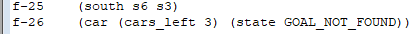
\includegraphics[scale=0.5]{images/facts_window_b1_2.png}

    \subsubsection{Κανόνας κίνησης}
    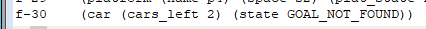
\includegraphics[scale=0.5]{images/facts_window_b1_3.png}

    \subsubsection{Μετά την εκκίνηση}
    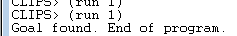
\includegraphics[scale=0.5]{images/dialog_window_b1_3.png}
    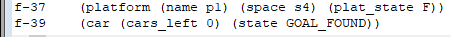
\includegraphics[scale=0.5]{images/facts_window_b1_4.png}

    \subsubsection{Σχόλια}
    \paragraph{}
    Εδώ βλέπουμε ότι φορτώνει τα γεγόντα και τους κανόνες χώρις πρόβλημα, διαβάζει από το πληκτρολόγιο πόσα αυτοκίνητα είναι στην λίστα, 
    αφαιρεί ένα αμάξι από την λίστα όταν το παρκάρει στην σωστή πλατφόρμα και τελείωνει όταν όλα τα αυτοκίνητα στην λίστα έχουν παρκάρει.
    Σε ένα άλλο ενδεικτικό τρέξιμο, με αυτοκίνητα πάνω από 5, το πρόγραμμα μπαίνει σε loop αφού δεν υπάρχει τρόπος να παρκάρει τα έξτρα αυτοκίνητα.

    \newpage
    \section{Παρατηρήσεις ενδιάμεσα των βήματων}
    \paragraph{}
    Από ότι φαίνεται, αυτός ο τρόπος λυσής συγκριτικά με τον άλλον τρόπο λύσης του πρώτου μερούς της εργασίας είναι τυχαίος και ίσως πιο αργός.
    Στην υλοποίηση, όμως, είναι πολύ πιο εύκολος, όποτε είναι πιο απλός για τον προγραμματιστή. Μπορεί να κολλήσει και να μην βρει πότε λύση,
    που δεν φαντάζομαι να είναι εφικτό αυτό στον προγραματικό κόσμο.

    \section{Βήμα 2}
    \subsection{Ζητούμενα δεύτερου βήματος}
    \paragraph{}
    Το βήμα 2 μας ζητάει να κάνουμε μια προέκταση του πρώτο βήματος, δηλαδή θα προσθέσουμε δύο παραπάνω όροφους, με ξεχωριστά spaces και platforms.
    Ο δεύτερος όροφος έχει τα spaces s7 εώς s12, όπου ο s7 και ο s12 είναι άδεια ενώ οι υπόλοιποι έχουν τις πλατφόρμες p6 εώς p9.
    Ο τρίτος όροφος έχει τα spaces s13 εώς s18, όπου ο s13 είναι άδειος και οι υπόλοιποι έχουν τις πλατφόρμες p10 εώς p14.
    Θα μπορεί να αλλάζει όροφο από τα spaces s5, s11 και το s17 με την χρήση ενός ανελκυστήρα.
    Επιπρόσθετα, μας ζητάει όποτε μπαίνει ένα νέο αμάξι να δίνουμε τον αριθμό κυκλοφορίας του με σκόπο να μπορούμε μετά να το εντωπίζουμε
    και να το ξεπαρκάρουμε με ακριβώς την αντίθετη διαδικασία.

    \subsection{Τι μπορούμε να χρησιμοποιήσουμε από το πρώτο βήμα}

    \begin{itemize}
        \item Τα templates του πρώτου βήματος
        \item Τα γεγονόντα του πρώτου βήματος
        \item Οι κανόνες του πρώτου βήματος
    \end{itemize}

    \paragraph{}
    Παρόλου που είναι σχεδόν έτοιμα, θα πρέπει να τα τροποποιήσουμε λίγακι.

    \subsubsection{Τροποποιήμενα templates πρώτου βήματος}
    \begin{lstlisting}
(deftemplate info
    (slot cars_left)
    (slot current_space)
    (slot state)
)
    \end{lstlisting}
    \paragraph{}
    To template car μετανομάστηκε σε info.

    \subsubsection{Τροποποιήμενα γεγονόντα πρώτου βήματος}
    \begin{lstlisting}
(deffacts space-init
    (space (name s1) (level 1) (state Y))
    (space (name s2) (level 1) (state N))
    (space (name s3) (level 1) (state Y))
    (space (name s4) (level 1) (state Y))
    (space (name s5) (level 1) (state Y))
    (space (name s6) (level 1) (state Y))
    (space (name s7) (level 2) (state N))
    (space (name s8) (level 2) (state Y))
    (space (name s9) (level 2) (state Y))
    (space (name s10) (level 2) (state Y))
    (space (name s11) (level 2) (state Y))
    (space (name s12) (level 2) (state N))
    (space (name s13) (level 3) (state N))
    (space (name s14) (level 3) (state Y))
    (space (name s15) (level 3) (state Y))
    (space (name s16) (level 3) (state Y))
    (space (name s17) (level 3) (state Y))
    (space (name s18) (level 3) (state Y))
)

(deffacts plat-init
    (platform (name p1) (space s1) (plat_state E))
    (platform (name p2) (space s3) (plat_state E))
    (platform (name p3) (space s4) (plat_state E))
    (platform (name p4) (space s5) (plat_state E))
    (platform (name p5) (space s6) (plat_state E))
    (platform (name p6) (space s8) (plat_state E))
    (platform (name p7) (space s9) (plat_state E))
    (platform (name p8) (space s10) (plat_state E))
    (platform (name p9) (space s11) (plat_state E))
    (platform (name p10) (space s14) (plat_state E))
    (platform (name p11) (space s15) (plat_state E))
    (platform (name p12) (space s16) (plat_state E))
    (platform (name p13) (space s17) (plat_state E))
    (platform (name p14) (space s18) (plat_state E))
)
    \end{lstlisting}

    \newpage
    \subsubsection{Τροποποιήμενοι κανόνες πρώτου βήματος}

    \begin{lstlisting}[caption=Τροποποιήμενος γενικός κανόνας κίνησης]
(defrule moveEast
    ?z<-(space (name ?y) (state N))
    (east ?y ?x)
    ?p<-(space (name ?x) (state Y))
    ?q<-(platform (name ?pn) (space ?x) (plat_state ?ps))
    ?c<-(info (cars_left ?cars) (current_space ?y) (state GOAL_NOT_FOUND)) ; Koitame kai to space pou eimaste twra
=>
    (modify ?p (state N))
    (modify ?z (state Y))
    
    (if (eq ?ps F)
    then
        (modify ?q (space ?y))
        (modify ?c (current_space ?x))
    
    else
        (printout t "Enter the license plate." crlf)
        (bind ?lp(read))
        (assert (car (license_plate ?lp) (platform ?pn)))
        (modify ?q (space ?y) (plat_state F))
        (modify ?c (cars_left (- ?cars 1)) (current_space ?x) (state PROMPT)) ; State pou mas paei sto prompt
    )
)
    \end{lstlisting}
    
    \paragraph{}
    Μπορούμε να δούμε ότι έχουμε προσθέσει ένα παραπάνω slot το οποίο κοιτάει το τρέχον space στο όποιο βρίσκεται
    αυτή την στιγμή ο αυτόματος παρκαδόρος. Αυτό γίνεται, επείδη πλέον έχουμε παραπάνω από ένα empty space, και
    κάπως θα πρέπει να το ξεχωρίζουμε ποιο είναι αυτό στο οποίο βρίσκεται ο παρκαδόρος. Επιπλέον, παρατηρούμε ότι
    όταν βάζουμε το αυτοκίνητο, ζητάμε από τον χρήστη να μας δώσει τον αριθμό κυκλοφορίας του και επείσης αλλάζει το state
    σε prompt.

    \subsection{Templates δεύτερου βήματος}
    \paragraph{}
    Αυτά είναι τα templates του δεύτερου βήματος:

    \begin{lstlisting}
(deftemplate car_to_find
    (slot license_plate)
)

(deftemplate car
    (slot license_plate)
    (slot platform)
)
    \end{lstlisting}

    \subsection{Γεγονόντα δεύτερου βήματος}
    \paragraph{}
    Αυτά είναι τα γεγονόντα του δεύτερου βήματος:

    \begin{lstlisting}
(deffacts up
    (up s5 s11)
    (up s11 s17)
)

(deffacts down
    (down s11 s5)
    (down s17 s11)
)
    \end{lstlisting}

    \subsection{Κανόνες δεύτερου βήματος}
    Τώρα θα δούμε αναλυτικά τους κανόνες του δεύτερου βήματος. Πλέον για τους κανόνες κινήσεις, αφού έχουμε πολυεπίπεδικο parking με διαφόρους
    όροφους, δεν μας φτάνει να μπορεί να πηγαίνει ανατολικά, βορεία, νότια και δυτικά αλλά και πάνω και κάτω. Οπότε, προσθέσαμε δύο παραπάνω
    κανόνες κίνησεις για κάθε τυπικό κανόνα που ύπαρχει.

    \subsubsection{Κανόνας prompt}
    \begin{lstlisting}[caption=Κανόνας prompt]
; Kanonas pou rwtaei ton xristi ean thelei na kseparkarei autokinhto
(defrule prompt
    (declare (salience 100))
    ?c<-(info (state PROMPT))
=>
    (printout t "Do you want to remove a car? y/n" crlf)
    (bind ?qu(read))
    (if (eq ?qu y)
    then
        (printout t "Give license plate." crlf)
        (bind ?lp(read)) ; Ean nai, tote pairnei to license plate kai arxizei na to psaxnei
        (modify ?c (state SEARCH_CAR))
        (assert (car_to_find (license_plate ?lp)))

    else
        (modify ?c (state BACK_TO_S2)) ; Ean oxi, tote gurnaei pisw sto s2
    )
)
    \end{lstlisting}

    \paragraph{}
    Κανόνας που ρώταει από τον χρήστη εάν θέλει να ξεπαρκάρει κάποιο αυτοκίνητο. Εάν απαντήσει ναι, τότε του ζητάει τον αριθμό κυκλοφορίας
    του αυτοκινήτου και αλλάζει το state σε SEARCH\_CAR. Η προϋπόθεση για να δουλέψει αυτός ο κανόνας είναι να έχουμε state PROMPT,
    που το παίρνουμε όταν τοποτεθείται τουλάχιστον ένα αυτοκίνητο.

    \subsubsection{Τυπικός κανόνας επιστροφής στο s2}
    \begin{lstlisting}[caption=Τυπικός κανόνας επιστροφής στο s2]
(defrule backToS2East
    ?z<-(space (name ?y) (state N))
    (east ?y ?x)
    ?p<-(space (name ?x) (state Y))
    ?q<-(platform (space ?x))
    ?c<-(info (state BACK_TO_S2) (current_space ?y))
=>
    (modify ?p (state N))
    (modify ?z (state Y))
    (modify ?q (space ?y))
    (if (eq ?x s2)
    then
        (modify ?c (current_space ?x) (state GOAL_NOT_FOUND))

    else
        (modify ?c (current_space ?x))
    )
)
    \end{lstlisting}

    \paragraph{}
    Αυτός ο κανόνας είναι αρκετά παρόμοιος με τον τυπικό κανόνα κίνησης, με την διαφόρα ότι αντί να ψάχνει αδεία πλατφόρμα, ψάχνει το space που έχει
    όνομα s2. Εάν το βρει, δίνει το state GOAL\_NOT\_FOUND.

    \newpage
    \subsubsection{Τυπικός κανόνας εύρεσης αυτοκίνητου}
    \begin{lstlisting}[caption=Τυπικός κανόνας εύρεσης αυτοκίνητου]
(defrule findCarEast
    ?z<-(space (name ?y) (state N))
    (east ?y ?x)
    ?p<-(space (name ?x) (state Y))
    ?q<-(platform (name ?pn) (space ?x))
    ?car<-(car (license_plate ?lp) (platform ?pn)) ; Autokinhto pou vriskete sthn pn platforma kai exei lp license plate
    ?c<-(info (state SEARCH_CAR))
    ?cf<-(car_to_find (license_plate ?lpf)) ; Euresi lpf license plate
=>
    (modify ?p (state N))
    (modify ?z (state Y))
    (modify ?q (space ?y))
    (if (eq ?lp ?lpf)
    then
        (retract ?car ?cf) ; Afairesh autokinhtou apo thn lista
        (modify ?c (current_space ?x) (state BACK_TO_S2))
    
    else
        (modify ?c (current_space ?x))
    )
)
    \end{lstlisting}

    \paragraph{}
    Εδώ ψάχνουμε το αυτοκίνητο, όπου βρίσκεται σε μία πλατφόρμα pn. Για να ξεπαρκάρει το αυτοκίνητο θα πρέπει ο αριθμός κυκλοφορίας του
    να είναι ίσος με τον αριθμό κυκλοφορίας από το αυτοκίνητο που ψάχνουμε. Αφού το αφαιρέσει με την χρήση της εντολής retract, θα αλλάξει το
    state σε BACK\_TO\_S2 για να γυρίσουμε πίσω στο s2.

    \newpage
    \subsection{Βήμα 2 source code}
    \lstinputlisting[caption=Βήμα 2]{code/parking.clp}

    \newpage
    \subsection{Ενδεικτικά τρεξίματα του δεύτερου βήματος}
    \subsubsection{Κανόνας κίνησης}
    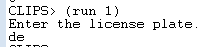
\includegraphics{images/dialog_window_b2_1.png}

    \subsubsection{Κανόνας prompt}
    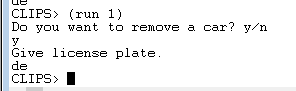
\includegraphics{images/dialog_window_b2_2.png}

    \section{Σχολιασμός - Βελτιώσεις}
    \paragraph{}
    Επείδη και στα δύο βήματα έχουμε τυχαία στρατηγική, πολλές φορές δεν λείγει το πρόγραμμα, ενώ αλλές φορές λείγει.

    \paragraph{}
    Από πλευράς βελτιώσεων, θα μπορούσα να χρησιμοποιούσα καλύτερη ονοματολογία των μεταβλήτων.

\end{document}